\documentclass[a4paper]{article}
\usepackage{sbc-template}
\usepackage[brazilian]{babel}
\usepackage[utf8]{inputenc}
\usepackage[T1]{fontenc}
\usepackage{enumerate}
\usepackage{color}
\usepackage{listings}
\usepackage{graphicx}
\usepackage{float}
\usepackage{hyperref}
\usepackage{amsmath}

\graphicspath{{figures/}}
\definecolor{dkgreen}{rgb}{0,0.6,0}
\definecolor{gray}{rgb}{0.5,0.5,0.5}
\definecolor{mauve}{rgb}{0.58,0,0.82}

\lstset{frame=tb,
	aboveskip=3mm,
	belowskip=3mm,
	showstringspaces=false,
	columns=flexible,
	basicstyle={\small\ttfamily},
	numbers=none,
	numberstyle=\tiny\color{gray},
	keywordstyle=\color{blue},
	commentstyle=\color{dkgreen},
	stringstyle=\color{mauve},
	breaklines=true,
	breakatwhitespace=true,
	language=matlab,
	tabsize=3
}

\sloppy

%
%Explicação do método de ponto fixo pelo Batista
%
%Um método iterativo simples consiste em resolver uma equação do tipo $x = \phi(x)$, aplicando sucessivamente a função $\phi$. De modo que, se a sequência $x_{n+1} = \phi(x_{n})$ for convergente, converge para uma solução da equação.

\author{Daniel De Luca, Diego Jornada, Matthias Nunes}

\address{Faculdade de Informática -- Pontifícia Universidade Católica do Rio Grande do Sul\\
  (PUCRS)
  \email{\{daniel.luca, diego.jornada, matthias.nunes\}@acad.pucrs.br}
}

\title{Métodos Computacionais \\ Trabalho I}

\begin{document}

\maketitle

\begin{resumo}

Este artigo descreve uma síntese sobre computação científica e alguns métodos
iterativos, quando utilizados para achar números irracionais.

\end{resumo}

\section{Introdução}

%Computação científica no brasil e no mundo.
Computação científica é a área que estuda a construção de modelos matemáticos e
técnicas para análises quantitativas para resolver problemas cinetíficos e de
engenharia.

\section{Métodos Iterativos}

Um \textbf{método iterativo} é um procedimento matemático para resolução de equações que gera uma sequência de aproximações, cada vez melhores, que servem como solução para uma classe de problemas. Uma implementação específica de um método iterativo, incluindo sua condição de parada, é um algoritmo. Um método iterativo é considerado \textbf{convergente} se a sequência de valores geradas converge para uma dada aproximação inicial.

Para uma definição mais teórica, o seguinte autor define:

\begin{quotation}
Um método iterativo consiste em repetir uma determinada operação um certo número de vezes até que nos seja fornecida uma aproximação, que satisfaça as condições do problema e, para tal, a sequência de valores deve ser convergente.\cite{batista2014metodos}

\end{quotation}

Nos problemas do tipo \emph{encontre a raíz da equação}, um método iterativo usa uma suposição inicial para gerar sucessivas aproximações à uma solução. Em Contraste, \textbf{métodos diretos} tentam resolver o problema em uma sequência \emph{finita} de operações.

Um método iterativo é formado por quatro partes:~\cite{claudio2000calculo}
\begin{enumerate}[a)]
	\item Estimativa inicial: uma ou mais aproximações para a raiz desejada.
    \item Atualização: uma fórmula que atualize a solução aproximada.
    \item Critério de parada: uma forma de estabelecer quando parar o processo iterativo em qualquer caso.
    \item Estimador de exatidão: está associado ao critério de parada e provê uma estimativa do erro cometido.
\end{enumerate}

\newpage

\section{Exercícios}
%PI = http://mathforum.org/library/drmath/view/65244.html
Nessa seção vamos encontrar números irracionais conhecidos utilizando métodos iterativos.

\subsection{Número de Ouro}

	O número de ouro, também conhecido como $\phi$, é o resultado da seguinte
	equação: $x^2-x-1$,existem algums algoritmos para realizar a aproximação
	neste artigo duas destas formas serão abordadas, a primeira utilizando
	frações continuas e o seguundo calculando as raizaes da equação utiizando
	método de newton.

\subsubsection{Frações Continuadas}

	Frações conitinuadas são formas de representar números reais de tal forma
	que a expressão básica tem o seguinte formato:

	$$\frac{b_1}{a_1 + \frac{b_2}{a_2 + \frac{b_3}{a_3 + \dots }}$$

Para encontrarmos o número de
ouro utilizamos o ambiente matemático \emph{octave}, e conseguimos gerar a
seguinte tabela:

\begin{table}[H]
	\centering
	\begin{tabular}{|c|c|c|c|}

		\hline
		Iteração & $x$ & Iteração & $x$ \\
		\hline
		1 & 2.00000000000000000000 & 26 & 1.61803398873830306393 \\
		\hline
		2 & 1.50000000000000000000 & 27 & 1.61803398875432247195 \\
		\hline
		3 & 1.66666666666666651864 & 28 & 1.61803398874820381081 \\
		\hline
		4 & 1.60000000000000008882 & 29 & 1.61803398875054060824 \\
		\hline
		5 & 1.62500000000000000000 & 30 & 1.61803398874964821097 \\
		\hline
		6 & 1.61538461538461541878 & 31 & 1.61803398874998904944 \\
		\hline
		7 & 1.61904761904761906877 & 32 & 1.61803398874985893130 \\
		\hline
		8 & 1.61764705882352943789 & 33 & 1.61803398874990866929 \\
		\hline
		9 & 1.61818181818181816567 & 34 & 1.61803398874988957346 \\
		\hline
		10 & 1.61797752808988759554 & 35 & 1.61803398874989690093 \\
		\hline
		11 & 1.61805555555555558023 & 36 & 1.61803398874989401435 \\
		\hline
		12 & 1.61802575107296142676 & 37 & 1.61803398874989512457 \\
		\hline
		13 & 1.61803713527851456000 & 38 & 1.61803398874989490253 \\
		\hline
		14 & 1.61803278688524576623 & 39 & 1.61803398874989490253 \\
		\hline
		15 & 1.61803444782168193150 & 40 & 1.61803398874989490253 \\
		\hline
		16 & 1.61803381340012508716 & 41 & 1.61803398874989490253 \\
		\hline
		17 & 1.61803405572755432118 & 42 & 1.61803398874989490253 \\
		\hline
		18 & 1.61803396316670644595 & 43 & 1.61803398874989490253 \\
		\hline
		19 & 1.61803399852180351814 & 44 & 1.61803398874989490253 \\
		\hline
		20 & 1.61803398501735795634 & 45 & 1.61803398874989490253 \\
		\hline
		21 & 1.61803399017559712547 & 46 & 1.61803398874989490253 \\
		\hline
		22 & 1.61803398820532517988 & 47 & 1.61803398874989490253 \\
		\hline
		23 & 1.61803398895790184753 & 48 & 1.61803398874989490253 \\
		\hline
		24 & 1.61803398867044334608 & 49 & 1.61803398874989490253 \\
		\hline
		25 & 1.61803398878024262686 & 50 & 1.61803398874989490253 \\
		\hline

	\end{tabular}
	\label{golden_fraction}
	\caption{Convergência do número de ouro pelo método de frações continuadas}
\end{table}

Como fica ilustrado na tabela, o número já se estabiliza antes mesmo de chegarmos à 50 iterações.

\begin{figure}[H]
    \centering
    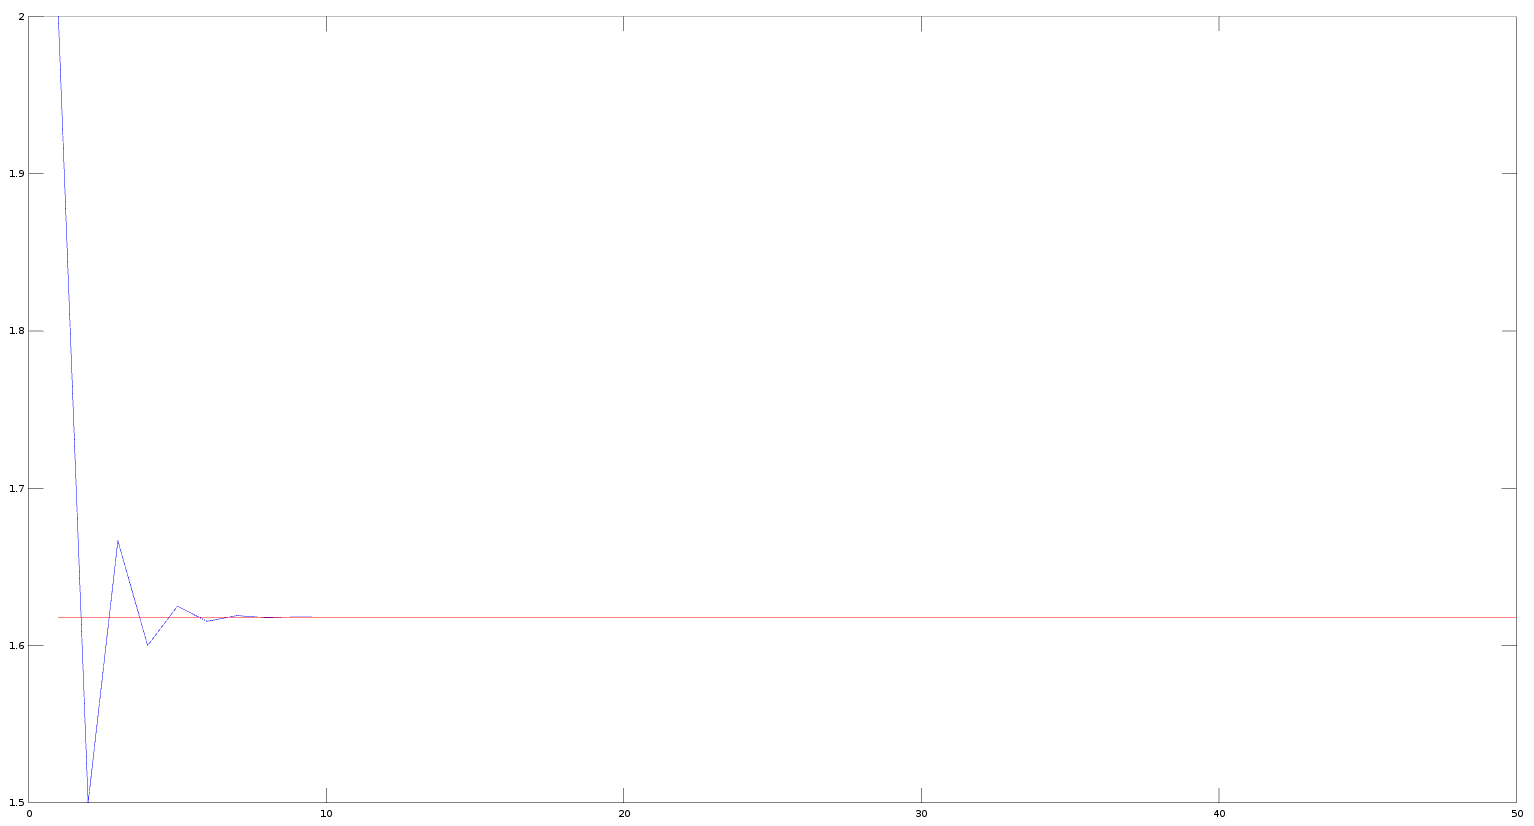
\includegraphics[width=100mm]{golden_frac.png}
    \caption{Convergência do número de ouro pelo método de frações continuadas}
    \label{golden_frac}
\end{figure}


O método iterativo utilizado foi descrito pelo seguinte código:

\begin{lstlisting}

function [x] =  phi_frac(iteration=1)
	aux = 1;
	for i= 1:iteration
		aux = double(1 + 1/aux);
		x(i) = aux;
	end
end

\end{lstlisting}

\subsubsection{Método de Newton}

A ideia do método de Newton é a seguinte: É estabelecido um chute inicial, que seja razoavelmente perto da raíz verdadeira, então a função é aproximada por sua reta tangente. O $x$ que intercepta a reta e a função é computado, e ele será uma melhor aproximação que o chute inicial. O método, então, pode ser iterado.

Analizando novamente o número de ouro, mas com o método de newton, um número muito menor de iterações é observado.

\begin{table}[H]
	\centering
	\begin{tabular}{|c|c|c|}
		\hline
		Iteração & $x$ & erro \\
		\hline
		1 & 1.66666666666666674068 & 0.33333333333333325932 \\
		\hline
		2 & 1.61904761904761906877 & 0.04761904761904767192 \\
		\hline
		3 & 1.61803444782168193150 & 0.00101317122593713727 \\
		\hline
		4 & 1.61803398874998904944 & 0.00000045907169288206 \\
		\hline
		5 & 1.61803398874989490253 & 0.00000000000009414691 \\
		\hline
		6 & 1.61803398874989490253 & 0.00000000000000000000 \\
		\hline
	\end{tabular}
	\label{golden_newton}
	\caption{Convergência do número de ouro pelo método de newton}
\end{table}

Isso pode ser observado no gráfico abaixo.

\begin{figure}[H]
    \centering
    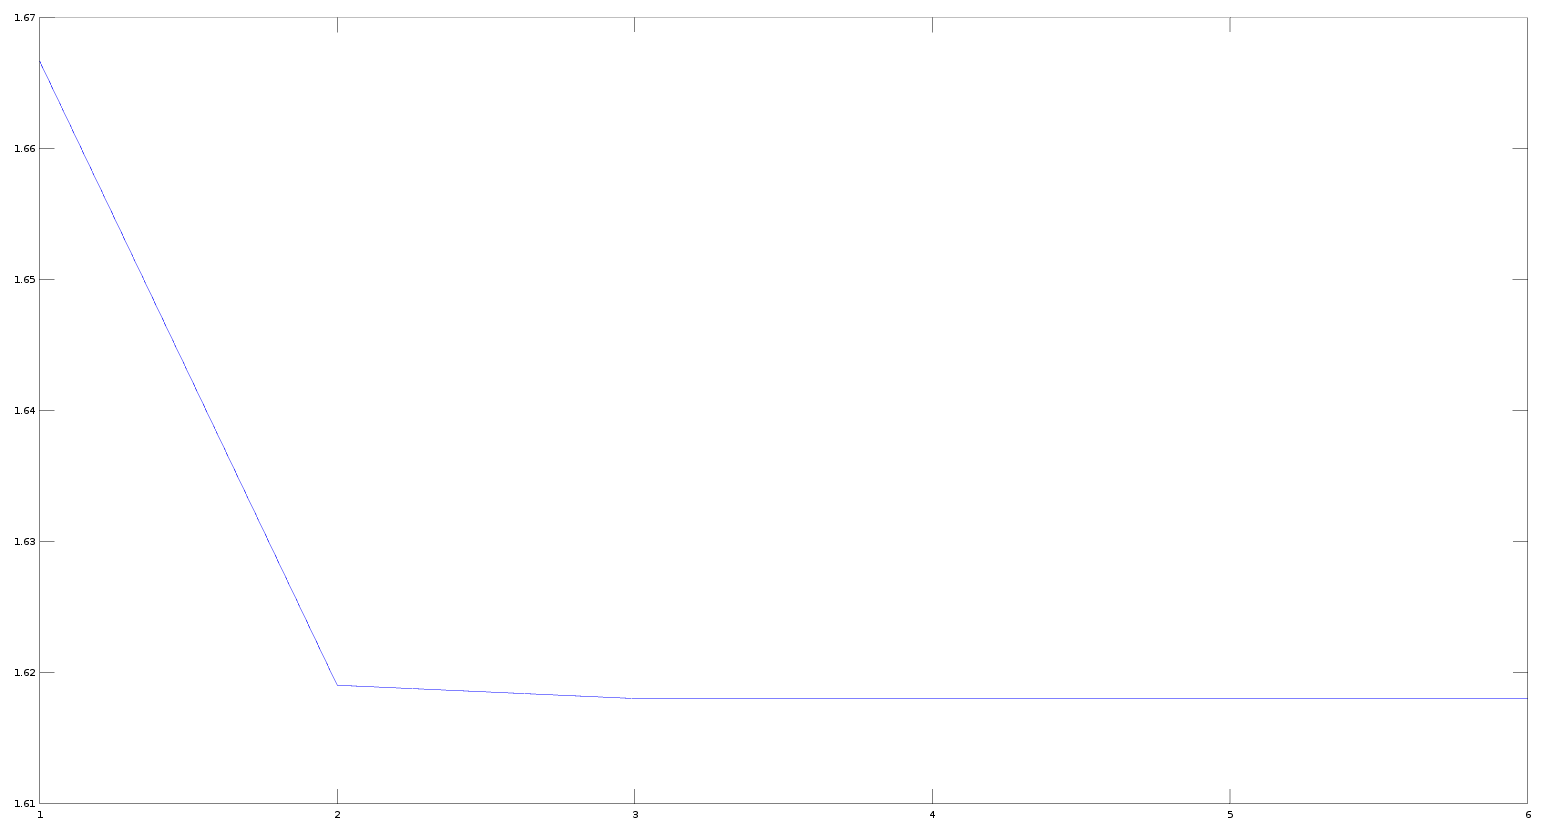
\includegraphics[width=100mm]{golden_newton.png}
    \caption{Convergência do número de ouro pelo método de newton}
    \label{golden_newton}
\end{figure}

O método iterativo utilizado foi descrito pelo seguinte código:

\begin{lstlisting}

function [x, ex] = newton( f, df, x0, tol, nmax)
	f = inline(f);
	df = inline(df);
	x(1) = double(x0 - (f(x0)/df(x0)));
	ex(1) = abs(x(1)-x0);
	k = 2;
	while k <= nmax && ex(k-1) > tol
		 x(k) = double(double(x(k-1)) - double((f(x(k-1))/df(x(k-1)))));
		 ex(k) = abs(x(k)-x(k-1));
		 k = k+1;
	end
end

\end{lstlisting}

\subsection{Pi($\pi$)}

\subsubsection{Método Misterioso}

Encontramos em um \href{http://mathforum.org/library/drmath/view/65244.html}{fórum de matemática} um método iterativo que calcula $\pi$ de uma forma aparentemente mais simples, apesar de sua complexidade estar escondida na função $sin$. O método está descrito a seguir:

\begin{equation}
P(n+1) = P(n) + sin(P(n))
\end{equation}

$P(n)$ seria a aproximação de $\pi$ na iteração $n$. Esse método consegue convergir para $\pi$ com um número muito baixo de iterações.

\begin{table}[H]
	\centering
	\begin{tabular}{|c|}
    	\hline
		$P(n)$ \\
		\hline
		3.14112000805986735230135309393517673015594482421875 \\
		\hline
		3.14159265357219563696844488731585443019866943359375 \\
		\hline
		3.14159265358979311599796346854418516159057617187500 \\
		\hline
		3.14159265358979311599796346854418516159057617187500 \\
		\hline
		3.14159265358979311599796346854418516159057617187500 \\
		\hline
		\hline
		$\pi$ \\
		\hline
		3.14159265358979311599796346854418516159057617187500 \\
		\hline
		\hline
		$P(n) - \pi$  Para visualizar a diferença \\
		\hline
		-4.72645529925763696610374609008431434631347656250000 \\
		\hline
		-1.75974790295185812283307313919067382812500000000000 \\
		\hline
		0.00000000000000000000000000000000000000000000000000 \\
		\hline
		0.00000000000000000000000000000000000000000000000000 \\
		\hline
		0.00000000000000000000000000000000000000000000000000 \\
		\hline
	\end{tabular}
	\label{pi_magic}
	\caption{Convergência do $\pi$}
\end{table}

O seguinte gráfico foi gerado com a análise dos result

\begin{figure}[H]
    \centering
    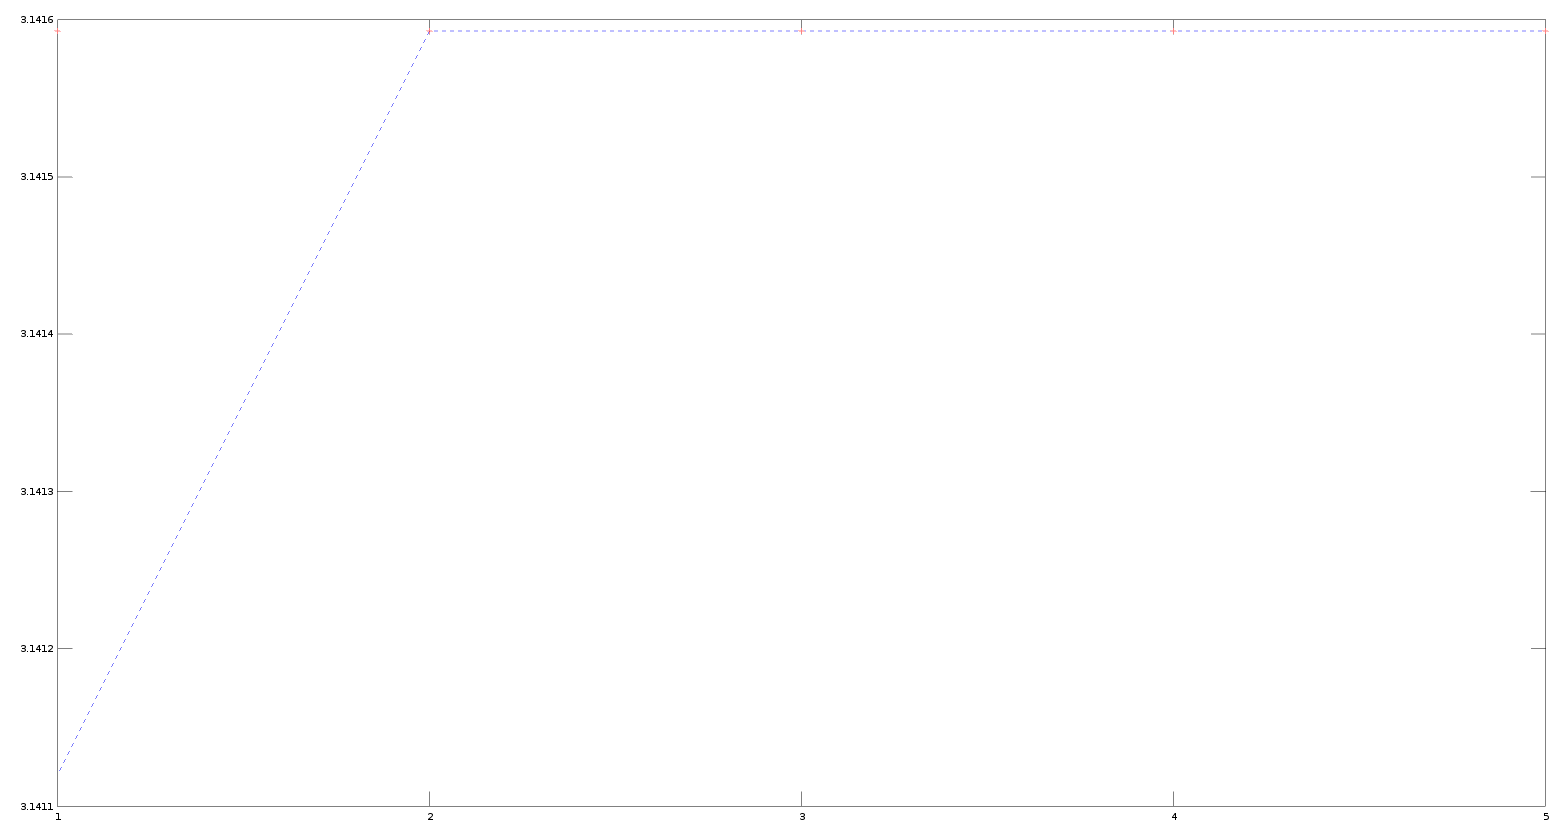
\includegraphics[width=100mm]{pi_magic.png}
    \caption{Convergência do $\pi$}
    \label{pi_magic}
\end{figure}

O método iterativo utilizado foi descrito pelo seguinte código:

\begin{lstlisting}

function [pif, pi_vec] = pi_it(iteration)
	pif(1) = 3 + sin(3);
	pi_vec(1) = pi
	for i = 2:iteration
		pif(i) = pif(i-1) + sin(pif(i-1));
		pi_vec(i) = pi;
		aux = pif(i);
	end
end

\end{lstlisting}



%\nocite{*}

\bibliographystyle{sbc}
\bibliography{sbc-template}

\end{document}
